\documentclass[11pt,a4paper]{article}

\usepackage{mathtools}
\usepackage{threeparttable}
\usepackage{longtable}
\usepackage{multirow}
\usepackage{booktabs}
\usepackage{changepage}
\usepackage{verbatim}
\usepackage{epigraph}
\usepackage{lscape}
\usepackage{pbox}
\usepackage{array}
\usepackage{natbib}
\usepackage{graphicx}
\usepackage{caption}


\linespread{1.5}
\graphicspath{{/Users/VK/Documents/Github/OECD-TiVA-LMIC-GVCs/misc/}}



\begin{document}

\section{Introduction}
The emergence of Global Value Chains (GVCs) offers a new path to industrialisation for developing countries. As \cite{riba12} phrases it, internationally fragmented production allows developing countries to join existing supply chains instead of building them. This brings about many potential advantages for these countries. Connecting with firms from advanced nations allows developing nations, for instance, to benefit from their sophisticated technologies and know-how. In addition, relying on an existing production network frees them from constraints imposed by economies of scale and the increased specialisation that GVCs imply limits the negative impact of unproductive parts of the domestic supply chain. After all, when competition moves from goods to tasks, comparative advantage becomes much finer and does not require a broad range of productive stages domestically. Conditional evidence for such a positive impact of GVC participation in low- and middle-income countries is presented in \citet{viku16} and \citet{unct13}.

Empirically, the considerable expansion of GVCs has been documented in several recent studies. For instance, \citet{dahuetal98, dahuetal01} show in two early seminal contributions that GVCs are responsible for a major share of the total growth in world trade from 1970 to 1990. Amongst others, \citet{rojoguno12a} and \citet{ribajalo13} find that this growth in GVC trade has even accelerated in the recent two decades. Furthermore, this work has not only revealed a rapid rise in production fragmentation across borders but it has also re-evaluated important indicators of trade, such as bilateral trade imbalances and revealed comparative advantage showing that calculating GVC indicators is central to a better understanding of countries' trade patters and competitiveness. 

A central step towards a more in-depth analysis of GVCs has been laid by \citet{rokoetal14} and \citet{zhwaetal13} who show that it is necessary to go beyond deriving origins of value added to examine production sharing comprehensively. They split goods into different categories and calculate metrics of how often these goods cross borders. This enables them to derive measures of GVC length but also allows to investigate how individual countries are integrated into GVCs. For instance, they show that a considerable part of US value added exports eventually returns home in the form of final goods which is indicative of the US being specialised in upstream production stages.\footnote{See \citeauthor{joamsoca15} (forthcoming) for a comprehensive review of the literature on GVCs and outsourcing.} 

However, these contributions typically have one of two shortcomings. Firstly, most evidence is based on data from high-income countries. The reason is that reliable time-series of both national and international input-output tables have only been available for this particular subset of countries. In addition, the evidence is regularly based on a small sample of GVC indicators that hide valuable information stemming from more decomposed and disaggregated indicators. 

In this paper we address these issues by applying the novel and more detailed gross export decomposition developed by \citet{zhwaetal13} and \citet{rokoetal14} to a new set of Inter-Country Input-Output tables (ICIOs) with extensive country coverage provided by the OECD. The new ICIOs allow us to get a better understanding of the GVC activities of low- and middle-income countries while the new decomposition allows us to zoom in more closely at these activities revealing information not available from standard GVC indicators.

Our analysis confirms the expansion of GVCs in recent years and presents evidence that GVCs have become longer over time. We also find that these developments are increasingly driven by low- and middle-income countries while the integration of high-income countries has begun to even out at a high level. In addition, we find that high-income countries typically are the starting and end points of GVCs in that they provide upstream inputs and then serve eventually again as demand markets for the final products. Low- and middle-income countries, on the other hand, are more specialised in downstream activities such as assembly and export typically less domestic value added. However, we observe that developing economies have begun to move upstream along the value chain and out of pure assembly occupying a wider set stages. This should allow them to generate more gains from GVC participation.

The paper is organised as follows. Section \ref{sec:data} reviews shortly the decomposition proposed by \citet[WWZ henceforth]{zhwaetal13} and outlines the new ICIOs provided by the OECD. Section \ref{sec:basics} discusses results using standard indicators and measures calculated with the new data while section \ref{sec:news} discusses the results for the novel indicators. Section \ref{sec:conclusion} concludes.



\section[New data and new indicators]{New data and new indicators\footnote{The following section draws heavily from \citet{zhwaetal13}, \citet{viku16}, and \cite{baquviku15}.}}\label{sec:data}

GVC analysis relies typically on Inter-Country Input-Output tables (ICIOs). ICIOs are matrices that give supply and demand relationships between industries within and across countries. For instance, ICIOs state the amount of inputs of the Indian steel industry in the output of the US car industry. However, for a correct examination of GVCs it is necessary to go a step further from the ICIOs by deriving the true value added origins of the US car output. If, for example, India depends on inputs from the US steel industry to supply the US car industry, then ICIOs overstate the actual contribution of India. The extension of the basic \citet{wale36} insight by \citet{dahuetal01} shows how the information in ICIOs can be decomposed to estimate such value added flows.

The idea is that the production of industry \textit{i} of country \textit{k} creates value added in industry $i$ itself, a direct contribution, but also in industries \textit{j} from \textit{k} or other countries \textit{l} that supply $i$ with inputs, an indirect contribution. Since these industries themselves rely on inputs, $i$'s production sets several rounds of indirect value added creation in motion that can mathematically be expressed as:
\begin{equation}
VB = V + VA + VAA + VAAA + ... = V (I+A+A^{2}+A^{3}+...),
\end{equation}
which, as an infinite geometric series with the elements of $A<1$, simplifies to
\begin{equation}
VB = V (I-A)^{-1},
\end{equation}
where \textit{V} is a matrix with the diagonal representing the direct value added contribution of each industry, \textit{A} is the Input-Output coefficient matrix, which means it gives the direct input flows between industries required for 1\$ of output, and $B = (I-A)^{-1}$ is the so called Leontief inverse. \textit{VB} gives thus so called value added multipliers, which denote the amount of value added that the production of an industry's 1\$ of output or exports brings about in all other industries. If we post-multiply $VB$ with exports, we get a matrix, $VAE$, with the elements being the value added origins of each industry's exports, $vae_{ikjl}$.
 
This basic decomposition has been widely used in GVC analysis since it allows the calculation of two informative GVC participation measures. Firstly, a backward linkage indicator that is given by the import content of exports, $i2e$, (\citet{dahuetal01}`s Vertical Specialisation) and calculated as follows:
\begin{equation}
i2e_{ik} = \frac{\sum_{l}{\sum_{j}vae_{jlik}}}{exports_{ik}} ,
\end{equation}
Secondly, a forward linkage indicator - \emph{e2r} (domestic content in foreign (re-)exports) - which is given by:
\begin{equation}\label{eq:dvar}
{e2r}_{ik} = \frac{\sum_{l}{\sum_{j} vae_{ikjl}}}{exports_{ik}} ,
\end{equation}
where \(l\  \neq k\).

These indicators can tell us how much a country is integrated into GVCs and if it acts mainly as a supplier or a user of foreign value added. However, the Leontief decomposition is only informative for the origin and destination of value added while ICIOs also contain info on the type of good that is being traded and and how often an intermediate crosses borders. The WWZ decomposition extends the Leontief decomposition in this direction and thereby extracts more insights from ICIOs.


\subsection{Wang-Wei-Zhu decomposition}\label{sub:wwz}

Since the derivation itself is not the focus of this paper, we present here only the final result for a $G$-country $N$-industry model (equation 37 in WWZ) and refer the interested reader to the original paper. WWZ use the Leontief decomposition and extend it using additional information from ICIOs on the final usage and destination of the exports (e.g. re-imported vs. absorbed abroad). This splits the exports, $E$, of industry $l$ in country $k$ into sixteen different parts broadly differentiated into the four broad categories domestic value added absorbed abroad, domestic value added returning home, foreign value added, and purely double counted terms:
\begin{align}\label{eq:wwz}
\begin{split}
E^{kl}
= &\left(V^k B^{kk} \right)^T * F^{kl} 
+ \left(V^k L^{kk} \right)^T * \left(A^{kl} B^{ll} F^{ll} \right)\\
+& \left(V^k L^{kk} \right)^T * (A^{kl} \sum_{t \neq k,l}^G  B^{lt} F^{tt} )
+ \left(V^k L^{kk} \right)^T *  (A^{kl} B^{ll} \sum_{t \neq k,l}^G  F^{lt} )\\ 
+&  \left(V^k L^{kk} \right)^T * (A^{kl} \sum_{t \neq k}^G \sum_{l,u \neq k,t}^G B^{lt} F^{tu} )
+ \left(V^k L^{kk} \right)^T * \left(A^{kl} B^{ll} F^{lk} \right)\\
+& \left(V^k L^{kk} \right)^T * (A^{kl} \sum_{t \neq k,l}^G  B^{lt} F^{tk} )
+ \left(V^k L^{kk} \right)^T * \left(A^{kl} B^{lk} F^{kk} \right) \\
+& \left(V^k L^{kk} \right)^T * (A^{kl} \sum_{t \neq k}^G  B^{lk} F^{kt} )
+ \left(V^k B^{kk} -  V^k L^{kk} \right)^T * \left(A^{kl} X^{l}  \right)\\
+& \left(V^l B^{lk} \right)^T * F^{kl}
+ \left(V^l B^{lk} \right)^T *  \left(A^{kl} L^{ll} F^{ll} \right)
+ \left(V^l B^{lk} \right)^T \\
*&  \left(A^{kl} L^{ll} E^{l*} \right) + (\sum_{t \neq k,l}^G  V^{t} B^{tk} )^{T} * F^{kl}
+ (\sum_{t \neq k,l}^G  V^{t} B^{tk} )^{T}\\
*&   \left(A^{kl} L^{ll} F^{ll} \right) + (\sum_{t \neq k,l}^G  V^{t} B^{tk} )^{T} *  \left(A^{kl} L^{ll} E^{l*} \right) ,
\end{split}
\end{align}
where $F$ is final demand, and $L$ refers to the domestic Leontief inverse as opposed to the global inverse $B$. $X$ is output while \textit{T} indicates a matrix transpose operation. 

The four main categories are further divided according to their final destination so that the final decomposition is given by:

\begin{itemize}
\item Domestic value added absorbed abroad (\textit{VAX\_G}, T1-5)
\begin{itemize}
\item Domestic value added in final exports (\textit{DVA\_FIN}, T1)
\item Domestic value added in intermediate exports (\textit{DVA\_INT}, T2-5)
\begin{itemize}
\item Domestic value added in intermediate exports absorbed by direct importers (\textit{DVA\_INT}, T2)
\item Domestic value added in intermediate exports re-exported to third countries (\textit{DVA\_INTrex}, T3-5)
\begin{itemize}
\item Domestic value added in intermediate exports re-exported to third countries as intermediate goods to produce domestic final goods (\textit{DVA\_INTrexI1}, T3)
\item Domestic value added in intermediate exports re-exported to third countries as  final goods (\textit{DVA\_INTrexF}, T4)
\item Domestic value added in intermediate exports re-exported to third countries as intermediate goods to produce exports (\textit{DVA\_INTrexI2}, T5)
\end{itemize}
\end{itemize}
\end{itemize}
\item Domestic value added returning home (\textit{RDV}, T6-8)
\begin{itemize}
\item Domestic value added returning home as final goods (\textit{RDV\_FIN}, T6)
\item Domestic value added returning home as final goods through third countries (\textit{RDV\_FIN2}, T7)
\item Domestic value added returning home as intermediate goods (\textit{RDV\_INT}, T8)
\end{itemize}
\item Foreign value added (\textit{FVA}, T11-12/14-15 )
\begin{itemize}
\item Foreign value added in final good exports (\textit{FVA\_FIN}, T11/14)
\begin{itemize}
\item Foreign value added in final good exports sourced from direct importer (\textit{MVA\_FIN}, T11)
\item Foreign value added in final good exports sourced from other countries (\textit{OVA\_FIN}, T14)
\end{itemize}
\item Foreign value added in intermediate good exports (\textit{FVA\_INT}, T12/15)
\begin{itemize}
\item Foreign value added in intermediate good exports sourced from direct importer (\textit{MVA\_INT}, T12)
\item Foreign value added in intermediate good exports sourced from other countries(\textit{OVA\_INT}, T15)
\end{itemize}
\end{itemize}
\item Pure double counting (\textit{PDC}, T9-10/13/16)
\begin{itemize}
\item Pure double counting from domestic source (\textit{DDC}, T9-10)
\begin{itemize}
\item Due to final goods exports production (\textit{DDF}, T9)
\item Due to intermediate goods exports production (\textit{DDI}, T10)
\end{itemize}
\item Pure double counting from foreign source (\textit{FDC}, T13/16)
\begin{itemize}
\item Due to direct importer exports production (\textit{FDF}, T13)
\item Due to other countries' exports production (\textit{FDI}, T16)
\end{itemize}
\end{itemize}
\end{itemize}

For the analysis, we use $dva\_fin$, $fva\_fin$, $rdv$, $pdc$ and the two aggregate measures $dva_inter$ combining $dva_int$ and $ddc$ as well as $fva_inter$ combining $fva_int$ and $fdc$. This collapses the indicator to a intuitive and manageable amount. 

The advantage of such a detailed decomposition is that these new indicators can inform us on how countries integrate into GVCs while the basic Leontief decomposition mainly informs us on the intensity of integration. High amounts of foreign value added in final goods exports are, for instance, suggestive of a specialisation in downstream tasks that add little value to a good, such as assembly. High amounts of domestic value added in intermediate exports, on the other hand, are evidence of a more upstream specialisation in tasks that add a lot of value, such as business services. By tracking these two variables over time we can then see which countries have succeeded in moving up the value chain. We will explain the indicators in more detail in combination with the decomposition results to facilitate the understanding.

Finally, it is necessary to point out that the high resolution of the WWZ decomposition does not mean that the Leontief decomposition does not contain valuable information at all. In fact, we exploit the decomposition of exports into source industry and source country by calculating variants of the standard indicators based on different characteristics. In particular, we will assess the integration of low- and middle-income countries into GVCs by computing the amount of value added that they supply for total GVC trade.


\subsection{OECD ICIOs}\label{sub:icios}
We use the new OECD ICIOs as the main data source for the GVC indicators and the industry position indicators. The OECD ICIOs constitute the most recent and most advanced release of Inter-Country Input-Output tables. The new version of the database provides ICIOs covering 61 countries and 34 industries for the years 1995, 2000, 2005, and 2008 to 2011.\footnote{Countries and industries are listed in the Appendix.}\textsuperscript{,}\footnote{Note that in the analysis 2009 and 2010 are excluded due to the global crisis.} This extensive country coverage is crucial for analysing how GVCs affect countries at different stages of development over time, a feature that has not been possible due to limited data availability in previous databases. The empirical literature discussed above shows that especially the extended coverage of Asia is important. To create ICIOs, the OECD combines national IO tables with international trade data. As OECD countries have a harmonised construction methodology, potential discrepancies between national IO tables should be minor. Furthermore, the advanced harmonisation across countries reduces the use of proportionality assumptions to derive the ratio of imported intermediates in an industry's demand to a minimum. In addition, the OECD has used elaborate techniques to deal with China's processing trade. Due to China's outstanding role in GVCs and processing trade, this implies a significant improvement for the reliability of the database.\footnote{See \citet{rokoetal12} for an analysis of China's processing trade.}



\section{What we know: Old facts with new data}\label{sec:basics}

In this section we reassess with our extensive OECD ICIO dataset stylised facts on GVC integration that are typically based on smaller samples. We start by examining the development of our most basic measure of GVC integration, namely the amount of foreign value added in exports labeled by \citet{ribajalo13} as $i2e$.\footnote{Note that at the aggregate level forward ($e2r$) and backward ($i2e$) linkages are identical and thus we only look at one of the two measures.} It captures backward linkages into value chains and shows the well-known increase in GVC integration from 1995 to 2011. As illustrated in Figure \ref{fig:i2e_t}, the value of $i2e$ has grown by approximately 350\% and by 35\% as a share of total exports from around 17\% to over 23\%. Thus, countries rely for their export production increasingly on inputs produced abroad. The numbers are in line with similar findings by \citet{rojoguno12b} but their sample ends in 2009. It is then interesting to see that after the slump during the financial crises in 2009, GVCs have quickly recovered and already have started to exceed their pre-crisis levels in 2011.

Another way to examine the expansion of GVCs from 1995 to 2011 is to look at their length instead of their trade volume. WWZ propose to use the amount of double counted trade, $pdc$, as a proxy for GVC length since its value goes up the more back-and-forth trade occurs, which is equivalent to an increase in the number of production stages. They show that its value has increased for 40 selected countries. In Figure \ref{fig:pdc_t}, we observe in our larger sample similarly that $pdc$ as a share of total exports has increased over the examined period by 73\% and thus more than $i2e$. Therefore, GVCs do not only channel more trade but also have become longer over time.

\begin{figure}
\centering
\begin{minipage}{0.45\textwidth}
\vspace{0.8cm}
\centering
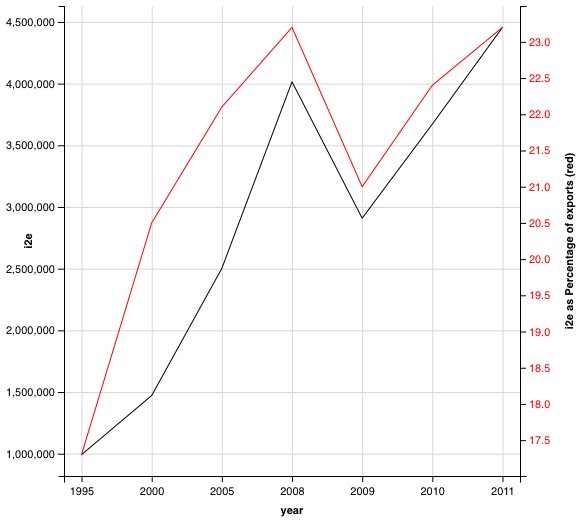
\includegraphics[width=\textwidth]{i2epercentage.png}
\caption{The development of GVC integration over time}
\label{fig:i2e_t}
\end{minipage}\hfill
\begin{minipage}{0.45\textwidth}
\centering
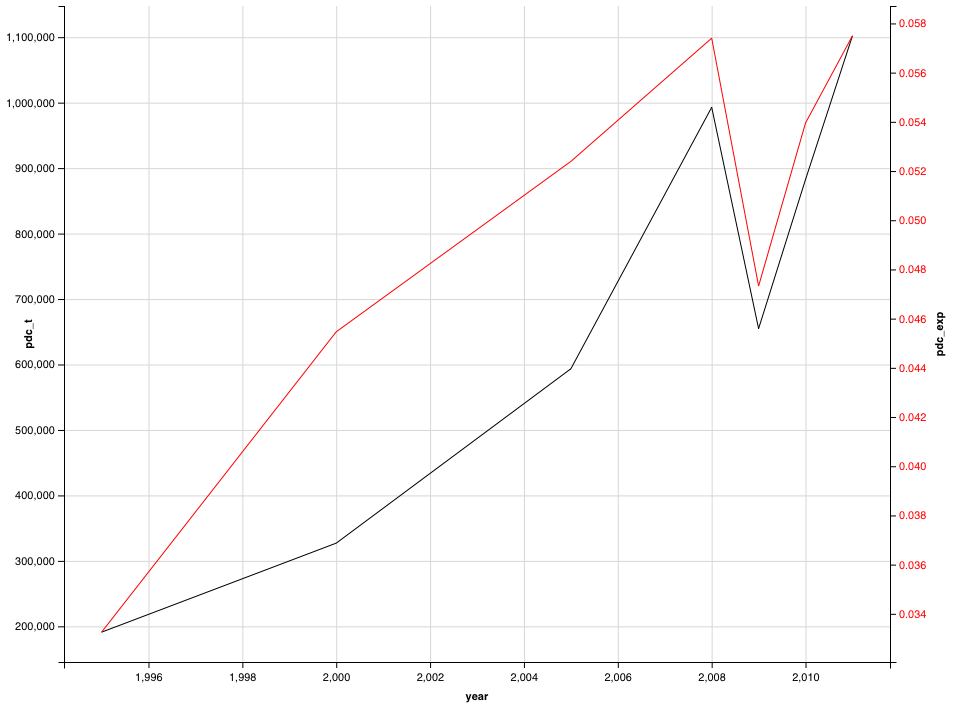
\includegraphics[width=\textwidth]{pdcII.png}
\caption{The development of double counted trade over time}
\label{fig:pdc_t}
\end{minipage}
\end{figure}

Turning from the development over time to sectoral differences in GVC integration, Figure \ref{fig:i2e_s} reveals in line with \citet{rojoguno12a} that the sectors exhibiting the highest degree of international fragmentation in terms of $i2e$ shares are heavy manufactures such as motor vehicles (MTR), other transport equipment (TRQ) and the metal industry (MET) as well as computers and electronics (CEQ and ELQ). In particular, the transport equipment and electronics industry are strongly engaged in GVCs having highly international production networks. For instance, Apple's iPhone contains inputs from 9 to 10 countries while the Boeing 787 production spans more than 5 countries. The sectors can be characterised as being close to final demand and producing complex differentiated goods. These characteristics can thus explain differences in GVC integration.

The bottom 6 industries in terms of $i2e$ shares are primary and services sectors such as agriculture (AGR), mining (MIN), R\&D and business services (BZS), or wholesale and retail trade (WRT). These sectors are typically located upstream in the supply chain far from final demand and have high value added to output ratios.

\begin{figure}
\centering
\begin{minipage}{0.45\textwidth}
\centering
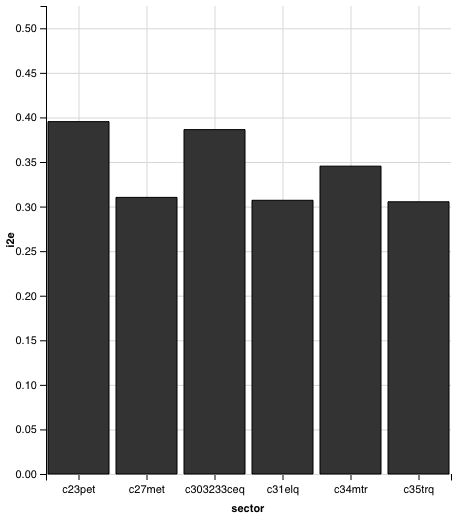
\includegraphics[width=\textwidth]{industries_i2e_top6.png}
\end{minipage}\hfill
\begin{minipage}{0.45\textwidth}
\centering
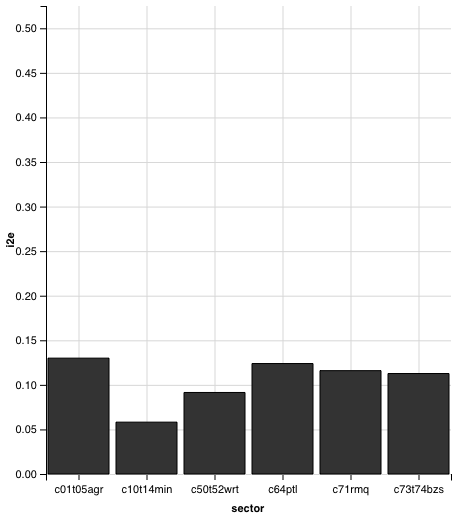
\includegraphics[width=\textwidth]{industries_i2e_bottom6.png}
\end{minipage}
\caption{Sectoral $i2e$ shares - Top and bottom 6.}
\label{fig:i2e_s}
\end{figure}

Naturally then, things are reversed when we look at the corresponding forward linkage GVC measure, $e2r$. It captures the amount of domestic value added in foreign exports and thus quantifies how important domestic industries are for foreign export production. Here, Figure \ref{fig:e2r_s} depicts that this indicator is dominated by the same upstream industries that are at the bottom of the $i2e$ ranking such as mining or business and telecommunication services (PTL). This shows that these industries are also strongly engaged in GVCs but their participation is of a different type. They primarily supply important inputs but do not serve final demand. 

With respect to services, it is also indicative of the servicification of manufacturing as described by \citet{ribaetal15}. This means that an increasing share of manufacturing gross exports is actually value added generated in services sectors and then embedded in the intermediate goods exports of manufacturers. This importance of services sectors for exports cannot be seen from standard gross trade statistics and thus constitutes a major advantage of trade in value added measures. 

It is also indicative of a growing internationalisation of services. More and more, services are being offshored and sourced from abroad. In that respect, it is also interesting to note that despite the low absolute $i2e$ shares, it is in services where a lot of the growth in $i2e$ has taken place. Five out of the six sectors with the highest growth in $i2e$ shares are services sectors.

\begin{figure}
\centering
\begin{minipage}{0.45\textwidth}
\centering
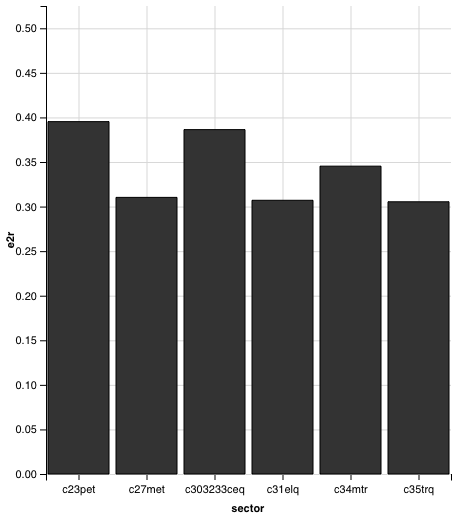
\includegraphics[width=\textwidth]{industries_e2r_top6.png}
\end{minipage}\hfill
\begin{minipage}{0.45\textwidth}
\centering
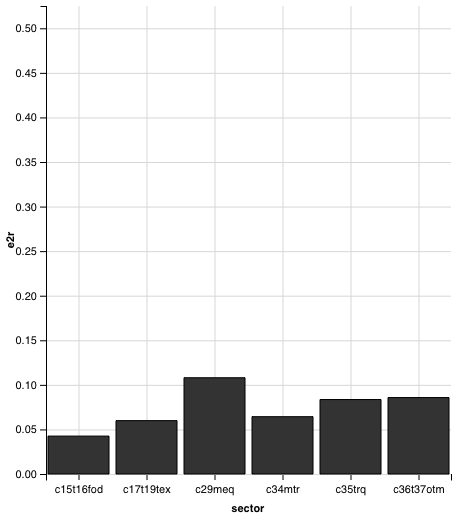
\includegraphics[width=\textwidth]{industries_e2r_bottom6.png}
\end{minipage}
\caption{Sectoral $e2r$ shares - Top and bottom 6.}
\label{fig:e2r_s}
\end{figure}

Finally, when we turn to differences in GVC integration by country we can confirm the findings by \citet{ribajalo13}. Figure \ref{fig:i2e_k} shows that small countries close to the major GVC hubs in Asia, Europe, and North America have the highest average $i2e$ shares. Examples include Malaysia and Slovakia. Countries specialised in the primary sector or assembly on the other hand have very low values. Correspondingly, Latin American countries with their focus on agriculture and mining have very weak backward linkages into GVCs. However, the development over time shows that some of the countries with the relatively low GVC integration have begun to catch up. For instance, Argentina, India and Turkey are in the top 6 when it comes to the growth of $i2e$ shares from 1995 to 2011.

Driven by the sectoral statistics, we then find again that for $e2r$ the picture is reversed with raw material exporters on top. If we abstract from these countries we find technologically advanced countries such as Switzerland and the main GVC hubs Japan, USA, and Germany to exhibit strong forward linkages into GVCs. In particular low and middle-income countries without raw materials such as Cambodia, Mexico, or Turkey have in contrast very weak linkages and have not been able to strengthen them significantly between 1995 and 2011.\footnote{The full set of results for $i2e$ and $e2r$ by country, and sector can be found in the Appendix. Since the results of WWZ decomposition are much more detailed the results not presented here are only available from the authors upon request.}

\begin{figure}[h]
\centering
\begin{minipage}{0.45\textwidth}
\centering
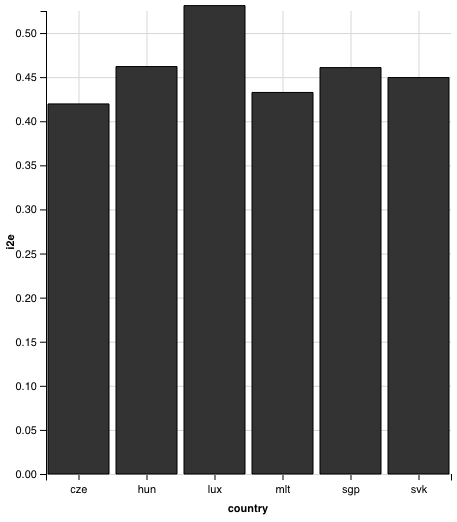
\includegraphics[width=\textwidth]{country_i2e_top_6.png}
\end{minipage}\hfill
\begin{minipage}{0.45\textwidth}
\centering
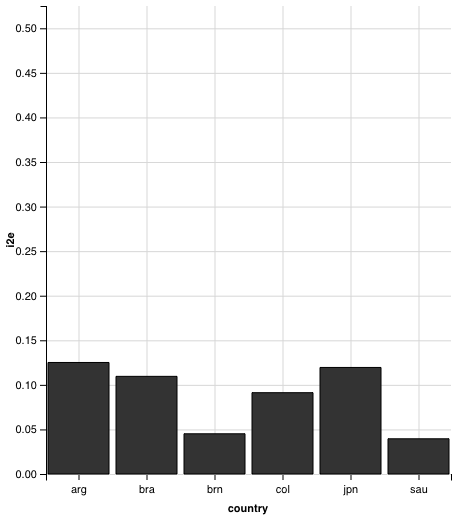
\includegraphics[width=\textwidth]{countries_i2e_bottom_6.png}
\end{minipage}
\caption{Countries' $i2e$ shares - Top and bottom 6.}
\label{fig:i2e_k}
\end{figure}

\begin{figure}[h]
\centering
\begin{minipage}{0.45\textwidth}
\centering
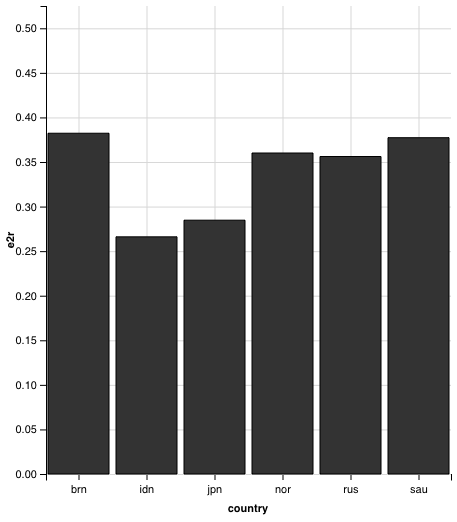
\includegraphics[width=\textwidth]{countries_e2r_top_6.png}
\end{minipage}\hfill
\begin{minipage}{0.45\textwidth}
\centering
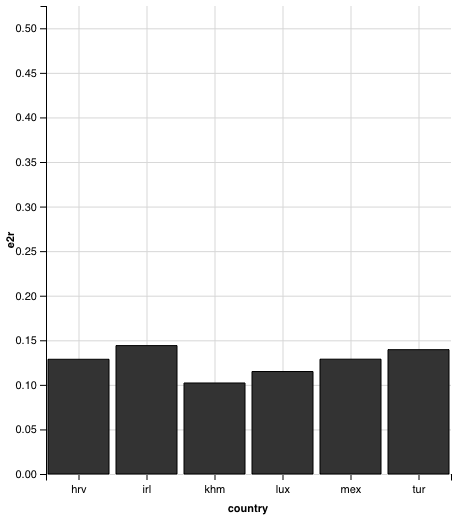
\includegraphics[width=\textwidth]{countries_e2r_bottom_6.png}
\end{minipage}
\caption{Countries' $e2r$ shares - Top and bottom 6.}
\label{fig:e2r_k}
\end{figure}



\section{The role of developing economies: New trends and patterns in GVCs}\label{sec:news}

The central advantage of our application is that we have new indicators for a new set of countries. This means we can not only confirm previous findings with a more representative sample but also provide several new insights. In particular, the OECD ICIO database extends the available list of countries in ICIOs by the following 21 regions: Argentina, Brunei Darussalam, Cambodia, Chile, Colombia, Costa Rica, Croatia, Hong Kong, Iceland, Israel, Malaysia, Norway, New Zealand, Philippines, Saudi Arabia, Singapore, Thailand, Tunisia, Vietnam, South Africa, and Switzerland. This means that in particular the coverage of low and middle income countries has increased considerably which allows us to analyse the GVC integration of developing economies in a much more detailed fashion than before.


\subsection{General trends in the GVC participation of developing economies}

Regarding the integration of low- and middle-income countries, \citet{rojoguno12a} have observed that per capita income is only a weak predictor for GVC integration due to the heterogeneity of economies in terms of size, industrial structure and location. In Table \ref{tab:gvc} we see that the average integration measured by either $i2e$ or $e2r$ does not vary strongly between income groups defined by the World Bank classification at the beginning of the sample period in 1995.\footnote{Note that in this section indicators are based only on manufacturing and services sectors to avoid spurious results stemming from primary sectors that are for technological reasons less integrated into GVCs.}
High-income economies have slightly stronger forward linkages but lower backward linkages which implies that their exports contain more domestic value added. Developing economies could thus try to upgrade their GVC integration by increasing domestic content in exports.

\begin{table}[htbp]\small
  \centering
  \caption{GVC integration by income}
    \begin{tabular}{lrrrr}
    \toprule
    Country group & \multicolumn{2}{c}{\textit{i2e}} & \multicolumn{2}{c}{\textit{e2r}} \\
          & \multicolumn{1}{c}{Average} & \multicolumn{1}{c}{$\Delta$ 95-11} & \multicolumn{1}{c}{Average} & \multicolumn{1}{c}{$\Delta$ 95-11} \\
              \midrule
    Low/Lower middle & 23.46\% & 48.22\% & 20.35\% & 38.58\% \\
    High & 22.64\% & 41.84\% & 21.85\% & 29.50\% \\
    \bottomrule
    \end{tabular}
  \label{tab:gvc}
    \caption*{Data is averaged across countries, sectors and years. $\Delta$ 95-11 refers to the growth of the \textit{i2e} and \textit{e2r} values from 1995 to 2011.}
\end{table}

Looking at the development over time, it is striking that the rise of GVC integration is increasingly driven by developing countries. The growth of both $i2e$ or $e2r$ has been much more pronounced in these economies as can be seen in Table \ref{tab:gvc}. In relative terms this means that the $i2e$ share of countries classified as low- or lower middle-income in total $i2e$ has increased from 9\% in 1995 to 24\% in 2011. Similarly, the $e2r$ share has increased from 9\% to 23\%.

Moreover, low- and lower middle-income countries do not only sell and source more from GVCs but they are also increasingly on the other side of the transaction. Figure \ref{fig:llmpartner} shows that the share of $i2e$ sourced from low- and lower middle-income countries has risen from 17\% to 33\% and the share of $e2r$ re-exported from them has expanded from 15\% to 28\%. Thus, developing countries have a large stake in GVCs and have moved from the periphery into the centre of these production networks.\footnote{However, we will see that GVC integration differs significantly among developing countries.}

\begin{figure}[h]
\centering
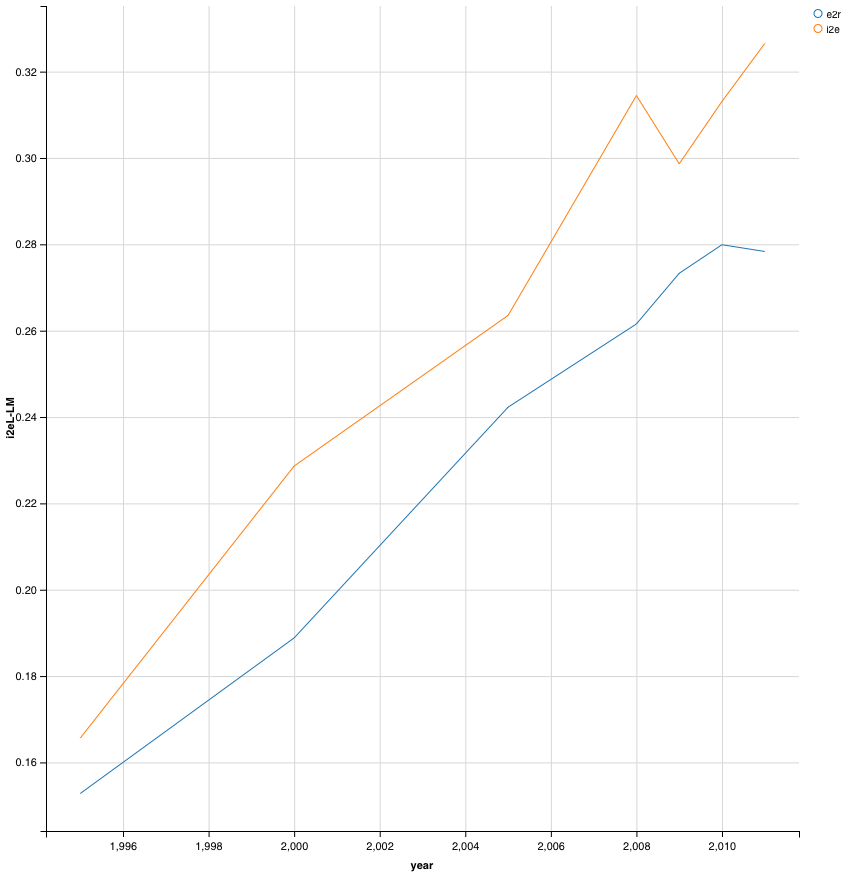
\includegraphics[width=0.5\textwidth]{e2r-i2e.png}
\caption{Share of value added sourced from (i2e) or sold to (e2r) low- and lower-middle income economies for export production.}
\label{fig:llmpartner}
\end{figure}

In a next step we zoom in and analyse the GVC participation of developing economies more closely with the help of the WWZ decomposition. As described in section \ref{sub:wwz}, WWZ show how the structure and changes in the structure of domestic and foreign content in exports inform us on a country's movement along the value chain. In particular, $i2e$ consists of foreign value added in final goods exports ($fva\_fin$), intermediate goods exports ($fva\_int$), and double counting ($fdc$). Table \ref{tab:wwz} shows that on average low- and lower middle-income countries have a higher share of $fva\_fin$ in $i2e$ (42\%) than high-income economies (39\%). This is in line with a specialisation of developing economies in downstream assembly tasks.

\begin{table}[htbp]\small
  \centering
  \caption{WWZ decomposition results by income}
    \begin{tabular}{lrrrrr}
    \toprule
    Country group & \multicolumn{1}{c}{\textit{fva\_fin}} & \multicolumn{1}{c}{\textit{fva\_inter}} & \multicolumn{1}{c}{\textit{dva\_fin}} & \multicolumn{1}{c}{\textit{dva\_inter}} & \multicolumn{1}{c}{\textit{rdv}} \\
    \midrule
    Low/Lower middle & 42.07\% & 57.93\% & 44.09\% & 54.73\% & 1.18\% \\
    High  & 39.38\% & 60.62\% & 40.73\% & 56.85\% & 2.42\% \\
    \bottomrule
    \end{tabular}
  \label{tab:wwz}
  \caption*{Data is averaged across countries, sectors and years. $fva$ variables are expressed as \% of $i2e$, $dva$ and $rdv$ variables as \% of domestic value added in total exports.}
\end{table}

However, a shift from foreign content in final goods to intermediate goods and double counted trade value would be indicative of moving up the value chain. For low- and lower middle-income countries, we indeed find as shown by Figure \ref{fig:llmwwz} that the share of $fva\_fin$ in $i2e$ has fallen by about 4\%. This gain accrues to the double counting part which goes up by 6\%. This means that production has become more fragmented and that developing economies increasingly occupy more upstream stages.

A similar exercise can be done for the domestic value added embodied in exports. The exported domestic value added of high-income countries tends to be dominated by intermediate goods (57\%) while low- and lower middle-income countries only achieve a value of 55\%. We obtain the same information when we look at the share of domestic value added that eventually returns home. Here, the value for high-income countries (2.42\%) is more than twice as high than its low- and lower-middle income counterpart (1.18\%), which indicates that high-income countries are located upstream in the value chain using developing economies for assembly. However, the data shows as well that developing economies have improved their position over time. The amount of domestic value added returning home has tripled from 1995 to 2011 and the share of final goods has decreased by more than 5\%. 

\begin{figure}
\centering
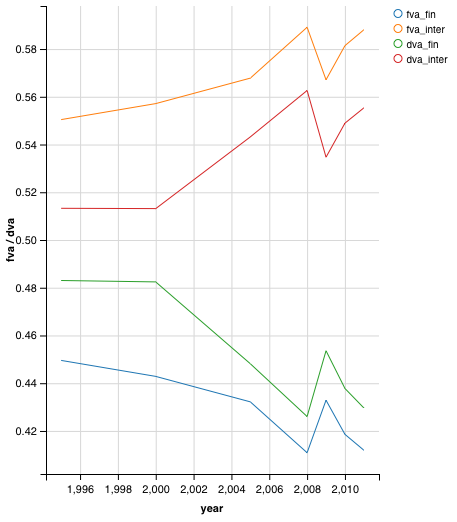
\includegraphics[width=0.5\textwidth]{fva-dva-fin-inter.png}
\caption{Development of developing economies' WWZ decomposition indicators over time.}
\label{fig:llmwwz}
\end{figure}

Thus, overall we get a clear picture that while developing economies are still positioned relatively more downstream in the value chain, they have succeeded to move up over the past two decades.



\subsection{Revealing new trends in the participation of developing economies}

The trends described in the previous section inform us on the average performance of developing countries but they might hide considerable heterogeneity among these countries. 
Therefore, we will merge a subset of the newly available countries into the three regions Central and South America (CSA), South East Asia (SEA), and Africa (AFR) and analyse the development of their GVC participation country by country. CSA covers Argentina, Chile, Colombia, and Costa Rica; SEA covers Cambodia, Malaysia, Philippines, Thailand, and Vietnam; while AFR covers South Africa and Tunisia.\\\

\textit{South East Asia}\\
The SEA economies for which data is newly available are Cambodia, Hong Kong, Malaysia, Philippines, Singapore, Thailand, and Vietnam. Since Singapore and Hong Kong are special cases due to their per capita income and size, we focus on Cambodia, Malaysia, Philippines, Thailand, and Vietnam. 

The two basic indicators of these countries, $i2e$ and $e2r$, presented in Table \ref{tab:seagvc} show that all five countries are primarily integrated into GVCs through backward linkages but in particular the Philippines have increased their forward linkages over the past two decades considerably. It also stands out that Cambodia and Vietnam have very low $e2r$ values suggesting a strong specialisation in low value added tasks located downstream in the chain. To obtain more detailed information on how these countries engage in GVCs we need however more disaggregated indicators.

The WWZ decomposition provides us with the necessary tools. We can see in Table \ref{tab:seawwz} that according to their high $fva\_fin$ values Cambodia and to a lesser extent Vietnam indeed perform mostly downstream tasks with typically low value added whereas Malaysia, Thailand, and the Philippines are positioned higher in the value chain exhibiting much lower $fva\_fin$ and $dva\_fin$ but higher $rdv$ values. Comparing these results to the analysis by WWZ, we find that the latter set of countries have a similar GVC integration structure to Indonesia but still are behind more advanced nations such as Korea and Taiwan. 

When we look at the change over time from 1995 to 2011, we see that Cambodia has actually moved into assembly with an increase of $fva\_fin$ of 35.2\%. This is in stark contrast to the remaining SEA countries which all achieved to move up the value chain. In particular, Vietnam is on a good path with the highest decline of $fva\_fin$ and might soon catch up with its local competitors regarding its position in GVCs. For Cambodia, on the other hand, this means that GVCs offer a major untapped potential for future growth. If the country manages to introduce more GVC-friendly policies it can leverage its location close to the GVC hubs China and Japan to continue on its successful growth path.\\

\begin{table}[!h]\small
  \centering
  \caption{GVC integration of SEA countries}
    \begin{tabular}{lrrrr}
    \toprule
    Country & \multicolumn{2}{c}{\multirow{1}[0]{*}{$i2e$}} & \multicolumn{2}{c}{\multirow{1}[0]{*}{$e2r$}} \\
    \multicolumn{1}{c}{} & \multicolumn{1}{c}{Average} & \multicolumn{1}{c}{$\Delta$ 95-11} & \multicolumn{1}{c}{Average} & \multicolumn{1}{c}{$\Delta$ 95-11} \\
    \midrule
    Cambodia & 39.4\% & 90.7\% & 8.4\% & -11.9\% \\
    Malaysia & 44.3\% & 37.1\% & 13.9\% & 10.2\% \\
    Philippines & 29.6\% & -20.7\% & 22.6\% & 105.0\% \\
    Thailand & 36.9\% & 64.3\% & 13.1\% & 20.2\% \\
    Vietnam & 38.3\% & 66.1\% & 10.6\% & 5.3\% \\
    \bottomrule
    \end{tabular}
  \label{tab:seagvc}
  \caption*{Data is averaged across sectors and years. $\Delta$ 95-11 refers to growth from 1995 to 2011.}
\end{table}

\begin{table}[!h]\small
  \centering
  \caption{WWZ decomposition results for SEA countries}
  \hspace*{-2.7cm}
    \begin{tabular}{lrrrrrrrrrr} 
    \toprule
    \multicolumn{1}{l}{\multirow{1}[0]{*}{Country}} & \multicolumn{2}{c}{$fva\_fin$} & \multicolumn{2}{c}{$fva\_inter$} & \multicolumn{2}{c}{$dva\_fin$} & \multicolumn{2}{c}{$dva\_inter$} & \multicolumn{2}{c}{$rdv$} \\
    \multicolumn{1}{l}{} & \multicolumn{1}{c}{Average} & \multicolumn{1}{c}{$\Delta$ 95-11} &
\multicolumn{1}{c}{Average} & \multicolumn{1}{c}{$\Delta$ 95-11} & \multicolumn{1}{c}{Average} & \multicolumn{1}{c}{$\Delta$ 95-11} & \multicolumn{1}{c}{Average} & \multicolumn{1}{c}{$\Delta$ 95-11} & \multicolumn{1}{c}{Average} & \multicolumn{1}{c}{$\Delta$ 95-11} \\
  \midrule
    Cambodia & 68.1\% & 35.2\% & 31.9\% & -35.7\% & 64.5\% & 26.8\% & 35.5\% & -27.5\% & 0.0\% & -29.7\% \\
    Malaysia & 39.3\% & -9.0\% & 60.7\% & 6.3\% & 40.8\% & -4.5\% & 58.9\% & 3.4\% & 0.4\% & -21.5\% \\
    Philippines & 35.5\% & -21.7\% & 64.5\% & 16.0\% & 38.9\% & -19.1\% & 60.9\% & 16.0\% & 0.2\% & 18.2\% \\
    Thailand & 41.4\% & -12.9\% & 58.6\% & 11.3\% & 47.4\% & -14.6\% & 52.3\% & 17.7\% & 0.3\% & 20.0\% \\
    Vietnam & 47.1\% & -22.6\% & 52.9\% & 30.0\% & 55.0\% & -9.0\% & 44.8\% & 12.7\% & 0.1\% & 103.4\% \\
    \bottomrule
    \end{tabular}
  \label{tab:seawwz}
   \caption*{Data is averaged across sectors and years. $fva$ variables are expressed as \% of $i2e$, $dva$ and $rdv$ variables as \% of domestic value added in total exports. $\Delta$ 95-11 refers to growth from 1995 to 2011.}
\end{table}


\textit{Central and South America}\\
The newly available CSA economies comprise Argentina, Chile, Colombia, and Costa Rica compared to previously only Mexico and Brazil. What stands out from looking at the standard GVC indicators presented in Table \ref{tab:csagvc} is that CSA is on average less integrated into GVCs than SEA and other developing regions. In particular, Argentina and Colombia have both very low backward and forward linkages highlighting the role of remoteness and sound policies as drivers of GVC integration. This is also mirrored in the fact that Chile and Costa Rica exhibit much higher GVC participation rates; albeit still below the SEA countries. These countries perform relatively well in several measures capturing a country's policy environment such as the World Bank's Doing Business Indicators or World Governance Indicators and, in the case of Costa Rica, are relatively closer to the North American GVC centre encompassing the USA, Canada, and Mexico. 

Focusing therefore on Costa Rica and Chile, we observe in Table \ref{tab:csawwz} that Chile's GVC integration structure starts to resembles the structure of high income countries. The major part of the country's integration is through intermediates as shown by the high $fva\_inter$ and $dva\_inter$ shares (78\% and 75\% respectively). However, the share of returned domestic value ($rdv$) is still much lower than the high-income average of 2.4\% and thus indicates that Chile is still in the process of catching up.

Costa Rica on the other hand possesses the typical GVC integration structure of lower middle-income economies with high $fva\_fin$ and $dva\_fin$ shares and a very small $rdv$ value of 0.02\%. Comparing the country to SEA, its structure resembles most closely the GVC integration of Vietnam. This comparison holds also when we look at Costa Rica's development over time, where we see a rapid expansion of $fva\_inter$, $dva\_inter$, and $rdv$ shares. The country is thus successfully moving up the value chain.

\begin{table}[htbp]\small
  \centering
  \caption{GVC integration of CSA countries}
    \begin{tabular}{lrrrr}
    \toprule
    Country & \multicolumn{2}{c}{\multirow{1}[0]{*}{$i2e$}} & \multicolumn{2}{c}{\multirow{1}[0]{*}{$e2r$}} \\
    \multicolumn{1}{c}{} & \multicolumn{1}{c}{Average} & \multicolumn{1}{c}{$\Delta$ 95-11} & \multicolumn{1}{c}{Average} & \multicolumn{1}{c}{$\Delta$ 95-11} \\
    \midrule
    Argentina & 13.4\% & 154.9\% & 13.4\% & 19.4\% \\
    Chile & 20.0\% & 44.8\% & 26.4\% & 35.4\% \\
    Colombia & 13.2\% & 15.2\% & 17.0\% & 45.5\% \\
    Costa Rica & 29.0\% & 21.1\% & 16.0\% & 60.8\% \\
    \bottomrule
\end{tabular}
  \label{tab:csagvc}
     \caption*{Data is averaged across sectors and years. $\Delta$ 95-11 refers to growth from 1995 to 2011.}

\end{table}

\begin{table}[htbp]\small
  \centering
  \caption{WWZ decomposition results for CSA countries}
  \hspace*{-2.7cm}
    \begin{tabular}{lrrrrrrrrrr} 
    \toprule
    \multicolumn{1}{l}{\multirow{1}[0]{*}{Country}} & \multicolumn{2}{c}{$fva\_fin$} & \multicolumn{2}{c}{$fva\_inter$} & \multicolumn{2}{c}{$dva\_fin$} & \multicolumn{2}{c}{$dva\_inter$} & \multicolumn{2}{c}{$rdv$} \\
    \multicolumn{1}{l}{} & \multicolumn{1}{c}{Average} & \multicolumn{1}{c}{$\Delta$ 95-11} &
\multicolumn{1}{c}{Average} & \multicolumn{1}{c}{$\Delta$ 95-11} & \multicolumn{1}{c}{Average} & \multicolumn{1}{c}{$\Delta$ 95-11} & \multicolumn{1}{c}{Average} & \multicolumn{1}{c}{$\Delta$ 95-11} & \multicolumn{1}{c}{Average} & \multicolumn{1}{c}{$\Delta$ 95-11} \\
  \midrule
    Argentina & 51.15\% & -6.33\% & 48.85\% & 7.95\% & 51.92\% & -5.71\% & 47.90\% & 7.01\% & 0.18\% & 49.61\% \\
    Chile & 22.23\% & -22.29\% & 77.77\% & 8.54\% & 24.61\% & -23.44\% & 75.25\% & 10.03\% & 0.14\% & 81.25\% \\
    Colombia & 39.41\% & -19.09\% & 60.59\% & 15.30\% & 39.32\% & -33.76\% & 60.55\% & 32.06\% & 0.12\% & 25.56\% \\
    Costa Rica & 45.99\% & -11.17\% & 54.01\% & 11.29\% & 50.97\% & -17.88\% & 49.01\% & 24.97\% & 0.02\% & 43.05\% \\
   \bottomrule
    \end{tabular}
  \label{tab:csawwz}
     \caption*{Data is averaged across sectors and years. $fva$ variables are expressed as \% of $i2e$, $dva$ and $rdv$ variables as \% of domestic value added in total exports. $\Delta$ 95-11 refers to growth from 1995 to 2011.}
\end{table}

\textit{Africa}\\
To conclude, we turn to Africa. GVC data on Africa is scarce and typically it is assumed that integration levels are low. However, the newly available OECD data comprises with Tunisia and South Africa two interesting and unique cases. Tunisia and South Africa offer relatively stable political environments and a relatively high degree of industrialisation which makes them two optimal case studies. Unlike many other African they do thus fulfil the basic requirements for GVC integration.

In line with this, Tables \ref{tab:afrgvc} and \ref{tab:afrwwz} show that in fact Tunisia has relatively high integration levels. Its integration pattern is very similar in both intensity, structure, and trend to Costa Rica and Vietnam. This means that Tunisia is mainly integrated through backward linkages and assembly tasks but is moving up the value chain. This is evidence that especially North Africa with its proximity to the European GVC hub can link into and benefit from GVCs.

South Africa is a different case since it is located far from most production networks and focuses primarily on raw materials. As a result, the country's integration levels are fairly low and more similar to Argentina and Colombia. Nevertheless, it is likely that it has benefitted from the boom in commodities caused by the rise of GVCs and the subsequent boost in global demand.

\begin{table}[htbp]\small
  \centering
  \caption{GVC integration of AFR countries}
    \begin{tabular}{lrrrr}
    \toprule
    Country & \multicolumn{2}{c}{\multirow{1}[0]{*}{$i2e$}} & \multicolumn{2}{c}{\multirow{1}[0]{*}{$e2r$}} \\
    \multicolumn{1}{c}{} & \multicolumn{1}{c}{Average} & \multicolumn{1}{c}{$\Delta$ 95-11} & \multicolumn{1}{c}{Average} & \multicolumn{1}{c}{$\Delta$ 95-11} \\
    \midrule
    South Africa & 21.3\% & 61.4\% & 19.9\% & 16.4\% \\
    Tunisia & 32.1\% & 35.6\% & 13.2\% & 33.1\% \\
\bottomrule
\end{tabular}
  \label{tab:afrgvc}
     \caption*{Data is averaged across sectors and years. $\Delta$ 95-11 refers to growth from 1995 to 2011.}
\end{table}

\begin{table}[htbp]\small
  \centering
  \caption{WWZ decomposition results for AFR countries}
  \hspace*{-2.7cm}
    \begin{tabular}{lrrrrrrrrrr} 
    \toprule
    \multicolumn{1}{l}{\multirow{1}[0]{*}{Country}} & \multicolumn{2}{c}{$fva\_fin$} & \multicolumn{2}{c}{$fva\_inter$} & \multicolumn{2}{c}{$dva\_fin$} & \multicolumn{2}{c}{$dva\_inter$} & \multicolumn{2}{c}{$rdv$} \\
    \multicolumn{1}{l}{} & \multicolumn{1}{c}{Average} & \multicolumn{1}{c}{$\Delta$ 95-11} &
\multicolumn{1}{c}{Average} & \multicolumn{1}{c}{$\Delta$ 95-11} & \multicolumn{1}{c}{Average} & \multicolumn{1}{c}{$\Delta$ 95-11} & \multicolumn{1}{c}{Average} & \multicolumn{1}{c}{$\Delta$ 95-11} & \multicolumn{1}{c}{Average} & \multicolumn{1}{c}{$\Delta$ 95-11} \\
  \midrule
South Africa & 48.76\% & -11.76\% & 51.24\% & 13.56\% & 54.43\% & -14.60\% & 45.49\% & 21.41\% & 0.08\% & 7.07\% \\
    Tunisia & 45.09\% & -14.97\% & 54.91\% & 15.19\% & 56.62\% & -4.47\% & 43.10\% & 5.56\% & 0.28\% & 147.59\% \\
\bottomrule
    \end{tabular}
  \label{tab:afrwwz}
     \caption*{Data is averaged across sectors and years. $fva$ variables are expressed as \% of $i2e$, $dva$ and $rdv$ variables as \% of domestic value added in total exports. $\Delta$ 95-11 refers to growth from 1995 to 2011.}
\end{table}



\section{Conclusion}\label{sec:conclusion}
GVCs are a major new factor in international trade. International production networks span across many countries and affect many industries while changing the way trade impacts domestic economies. This development requires new data and new statistics that appropriately capture countries' integration into GVCs. In this paper, we make use both such novelties in terms of data and statistics by applying a novel gross export decomposition methodology to a new expanded dataset.

More precisely, we apply the Wang-Wei-Zhu decomposition based on \citet{zhwaetal13} and \citet{rokoetal14} to a new set of Inter-Country Input-Output tables built by the OECD. The advantage is twofold. Firstly, the WWZ decomposition allows to analyse the structure of regions' GVC integration in addition to the intensity measures provided by previous decompositions leading to deeper insights into GVC integration patterns. Secondly, the new OECD ICIOs cover a much larger fraction of developing economies than previous ICIOs. This allows us to get a better understanding of how these countries integrate into GVCs.

We find that many ideas based on previous anecdotal evidence can be confirmed by the data. In particular, there is a central difference in the structure of high-income economies' integration into GVCs compared to developing economies when it comes to the position in GVCs. If we abstract from primary sectors, high-income economies are typically positioned more upstream in the value chain which can be seen from the concentration of their value added in intermediate goods exports. In addition, they also serve as market of final demand which can be seen from their relatively high share of exported domestic value added returning home eventually for final consumption.

Developing economies, on the other hand, tend to be positioned more downstream which can be deduced from the concentration of their GVC participation in final goods exports and the fact that their forward linkages and returning domestic value added tend to be low. These two stylised facts suggest that high-income economies use GVCs to outsource low value added downstream production stages and eventually reimport the final goods. However, when looking at the development over time it emerges strongly that many developing economies have succeeded in moving up the value chain and that the general trend points to a more even distribution of value added across the different countries.

Finally, we use the new data to look at selected low- and middle income economies in three different regions, namely South-East Asia, Latin America and the Caribbean, and Africa. South-East Asia has as expected the highest levels of GVC integration while we observe more heterogeneity in Latin America and the Caribbean where especially Chile and Costa Rica perform well. In Africa, we find that Tunisia has developed backward linkages into GVCs, which shows that Northern Africa has the potential to become part of the European GVC network.

Overall, we show that low- and middle-income countries have become an integral part of GVCs and are increasingly the driver of their expansion. In addition, they increasingly succeed in moving into higher value added stages of the production networks. While the exact implications of integration into GVCs are still being researched, it is clear that they offer significant potential for industrialisation and growth and therefore countries like the Philippines, Costa Rica, or Tunisia are in a good position and can serve as examples for comparable countries.


\clearpage

\bibliographystyle{chicago}
\bibliography{GVCandLMICs}

\clearpage

 \appendix
 
\section{Appendix}
\begin{table}[h]\small
  \centering
   \hspace*{-2.8cm}
    \begin{tabular}{lrrrrrr}
    \toprule
    \multicolumn{1}{l}{\textit{country}} & \multicolumn{1}{c}{\textit{Average (i2e values)}} & \multicolumn{1}{c}{\textit{Average (e2r values)}} & \multicolumn{1}{c}{\textit{Average (i2e)}} & \multicolumn{1}{c}{\textit{Average (e2r)}} & \multicolumn{1}{c}{\textit{$\Delta$ 95-11 (i2e)}} & \multicolumn{1}{c}{\textit{$\Delta$ 95-11  (e2r)}} \\
    \midrule
    arg   & 52,790 & 66,036 & 12.51\% & 15.65\% & 145.93\% & 30.04\% \\
    aus   & 178,117 & 343,084 & 13.35\% & 25.71\% & 18.21\% & 59.23\% \\
    aut   & 250,022 & 214,630 & 25.87\% & 22.21\% & 29.59\% & 39.90\% \\
    bel   & 437,578 & 285,355 & 32.53\% & 21.22\% & 10.66\% & 30.78\% \\
    bgr   & 51,393 & 19,864 & 38.01\% & 14.69\% & 32.70\% & 12.35\% \\
    bra   & 129,301 & 245,839 & 10.95\% & 20.83\% & 37.97\% & 57.77\% \\
    brn   & 2,412 & 20,438 & 4.51\% & 38.23\% & -41.34\% & 103.27\% \\
    can   & 647,662 & 407,957 & 23.54\% & 14.83\% & -3.54\% & 70.21\% \\
    che   & 334,258 & 343,657 & 21.84\% & 22.45\% & 23.45\% & 37.02\% \\
    chl   & 77,961 & 103,023 & 19.70\% & 26.03\% & 41.95\% & 42.06\% \\
    chn   & 1,831,434 & 1,293,766 & 24.07\% & 17.00\% & 62.57\% & 37.17\% \\
    col   & 21,746 & 57,971 & 9.12\% & 24.31\% & -9.63\% & 93.42\% \\
    cri   & 21,400 & 11,671 & 28.07\% & 15.31\% & 25.42\% & 48.66\% \\
    cyp   & 12,327 & 8,448 & 22.01\% & 15.09\% & 0.27\% & 53.75\% \\
    cze   & 290,027 & 129,166 & 41.96\% & 18.69\% & 48.79\% & 11.22\% \\
    deu   & 1,640,838 & 1,628,409 & 22.51\% & 22.34\% & 71.81\% & 13.06\% \\
    dnk   & 224,697 & 165,653 & 29.42\% & 21.69\% & 38.07\% & 43.47\% \\
    esp   & 546,406 & 383,881 & 25.13\% & 17.66\% & 39.96\% & 35.86\% \\
    est   & 21,777 & 11,992 & 34.90\% & 19.22\% & -3.58\% & 44.23\% \\
    fin   & 182,478 & 125,397 & 31.43\% & 21.60\% & 44.07\% & 6.99\% \\
    fra   & 888,006 & 773,925 & 23.01\% & 20.05\% & 44.76\% & 19.68\% \\
    gbr   & 766,576 & 909,659 & 19.52\% & 23.17\% & 25.71\% & 27.55\% \\
    grc   & 81,945 & 60,159 & 22.43\% & 16.47\% & 52.51\% & 51.65\% \\
    hkg   & 115,876 & 121,589 & 18.98\% & 19.92\% & -7.57\% & 53.77\% \\
    hrv   & 20,725 & 13,277 & 20.09\% & 12.87\% & -3.24\% & -4.93\% \\
    hun   & 236,208 & 78,585 & 46.20\% & 15.37\% & 59.55\% & 23.83\% \\
    idn   & 116,161 & 238,302 & 12.97\% & 26.61\% & -4.24\% & 96.09\% \\
    ind   & 356,692 & 298,471 & 21.34\% & 17.86\% & 178.40\% & 42.28\% \\
    irl   & 472,729 & 162,263 & 41.96\% & 14.40\% & 11.87\% & 19.69\% \\
    isl   & 11,301 & 8,977 & 29.32\% & 23.29\% & 84.40\% & 71.61\% \\
    \end{tabular}
\end{table}

\begin{table}[h]\small
  \centering
    \hspace*{-2.8cm}
    \begin{tabular}{lrrrrrr}
    \toprule
    \multicolumn{1}{l}{\textit{country}} & \multicolumn{1}{c}{\textit{Average (i2e values)}} & \multicolumn{1}{c}{\textit{Average (e2r values)}} & \multicolumn{1}{c}{\textit{Average (i2e)}} & \multicolumn{1}{c}{\textit{Average (e2r)}} & \multicolumn{1}{c}{\textit{$\Delta$ 95-11 (i2e)}} & \multicolumn{1}{c}{\textit{$\Delta$ 95-11  (e2r)}} \\
    \midrule
    isr   & 105,427 & 75,275 & 23.86\% & 17.04\% & 11.05\% & 53.19\% \\
    ita   & 778,367 & 641,040 & 23.21\% & 19.12\% & 53.48\% & 35.00\% \\
    jpn   & 582,907 & 1,388,524 & 11.95\% & 28.47\% & 164.46\% & 32.58\% \\
    khm   & 11,889 & 3,224 & 37.65\% & 10.21\% & 186.29\% & -36.76\% \\
    kor   & 1,034,054 & 521,202 & 37.70\% & 19.00\% & 88.43\% & 18.61\% \\
    ltu   & 16,707 & 15,497 & 22.83\% & 21.17\% & -4.03\% & 42.99\% \\
    lux   & 237,935 & 51,509 & 53.11\% & 11.50\% & 40.29\% & -15.58\% \\
    lva   & 14,530 & 13,063 & 25.95\% & 23.33\% & 25.01\% & 34.38\% \\
    mex   & 479,806 & 214,457 & 28.82\% & 12.88\% & 20.84\% & 31.28\% \\
    mlt   & 14,762 & 4,931 & 43.26\% & 14.45\% & -27.41\% & 108.31\% \\
    mys   & 517,084 & 215,738 & 41.45\% & 17.29\% & 33.36\% & 23.93\% \\
    nld   & 306,010 & 390,300 & 19.50\% & 24.87\% & -14.29\% & 51.12\% \\
    nor   & 163,813 & 351,592 & 16.78\% & 36.01\% & -13.46\% & 57.48\% \\
    nzl   & 39,712 & 33,912 & 17.08\% & 14.59\% & -0.73\% & 48.61\% \\
    phl   & 103,838 & 82,783 & 29.04\% & 23.15\% & -20.59\% & 101.26\% \\
    pol   & 273,027 & 198,877 & 29.34\% & 21.37\% & 99.99\% & 15.65\% \\
    prt   & 125,283 & 64,391 & 30.77\% & 15.81\% & 18.69\% & 37.51\% \\
    rou   & 59,385 & 54,956 & 24.23\% & 22.42\% & 14.95\% & 45.54\% \\
    rus   & 317,701 & 837,747 & 13.51\% & 35.62\% & 3.61\% & 56.47\% \\
    sau   & 57,392 & 547,987 & 3.95\% & 37.73\% & -15.39\% & 56.02\% \\
    sgp   & 548,286 & 219,149 & 46.08\% & 18.42\% & 12.95\% & 61.94\% \\
    svk   & 140,548 & 61,023 & 44.95\% & 19.52\% & 47.60\% & 7.80\% \\
    svn   & 51,465 & 29,065 & 34.78\% & 19.64\% & 11.26\% & 58.26\% \\
    swe   & 355,353 & 262,980 & 29.09\% & 21.52\% & 8.68\% & 29.44\% \\
    tha   & 391,773 & 156,527 & 36.05\% & 14.40\% & 61.19\% & 23.84\% \\
    tun   & 35,124 & 18,724 & 30.17\% & 16.08\% & 30.65\% & 48.33\% \\
    tur   & 180,927 & 113,136 & 22.30\% & 13.95\% & 195.25\% & 12.71\% \\
    twn   & 649,797 & 353,241 & 39.52\% & 21.48\% & 41.83\% & 60.53\% \\
    usa   & 1,318,846 & 2,248,028 & 13.52\% & 23.04\% & 30.75\% & 26.87\% \\
    vnm   & 119,821 & 57,005 & 33.76\% & 16.06\% & 72.69\% & 19.95\% \\
    zaf   & 102,394 & 122,842 & 19.31\% & 23.16\% & 47.60\% & 24.98\% \\
    \bottomrule
    \end{tabular}
      \caption{GVC indicators by country}
  \label{tab:gvc_k}
\end{table}

\begin{table}[h]\small
  \centering
    \hspace*{-3cm}
    \begin{tabular}{lrrrrrr}
    \toprule
    \multicolumn{1}{l}{\textit{sector}} & \multicolumn{1}{c}{\textit{Average (i2e values)}} & \multicolumn{1}{c}{\textit{Average (e2r values)}} & \multicolumn{1}{c}{\textit{Average (i2e)}} & \multicolumn{1}{c}{\textit{Average (e2r)}} & \multicolumn{1}{c}{\textit{$\Delta$ 95-11 (i2e)}} & \multicolumn{1}{c}{\textit{$\Delta$ 95-11  (e2r)}} \\
    \midrule
    c01t05agr & 227,969 & 364,681 & 13.00\% & 20.79\% & 36.13\% & 27.51\% \\
    c10t14min & 435,816 & 3,324,446 & 5.82\% & 44.38\% & -4.51\% & 55.66\% \\
    c15t16fod & 675,902 & 146,824 & 19.58\% & 4.25\% & 23.04\% & 32.73\% \\
    c17t19tex & 679,185 & 174,555 & 23.30\% & 5.99\% & 9.49\% & 2.72\% \\
    c20wod & 105,771 & 80,461 & 20.56\% & 15.64\% & 30.59\% & 63.12\% \\
    c21t22pap & 302,255 & 344,112 & 19.23\% & 21.89\% & 27.63\% & 7.10\% \\
    c23pet & 1,285,522 & 356,703 & 39.53\% & 10.97\% & 65.81\% & -8.04\% \\
    c24chm & 1,762,631 & 925,255 & 28.18\% & 14.79\% & 52.19\% & -2.18\% \\
    c25rbp & 446,528 & 309,253 & 27.89\% & 19.32\% & 38.26\% & 3.06\% \\
    c26nmm & 161,574 & 126,800 & 22.09\% & 17.34\% & 41.44\% & 17.72\% \\
    c27met & 1,340,507 & 868,120 & 31.03\% & 20.10\% & 36.53\% & -11.26\% \\
    c28fbm & 481,732 & 441,396 & 27.53\% & 25.23\% & 38.11\% & 6.86\% \\
    c29meq & 1,398,864 & 570,006 & 26.50\% & 10.80\% & 39.73\% & 30.96\% \\
    c303233ceq & 3,162,705 & 1,062,750 & 38.63\% & 12.98\% & 45.28\% & 18.74\% \\
    c31elq & 713,928 & 301,827 & 30.71\% & 12.98\% & 37.32\% & -3.42\% \\
    c34mtr & 1,827,519 & 340,198 & 34.53\% & 6.43\% & 33.39\% & 7.25\% \\
    c35trq & 745,063 & 203,834 & 30.54\% & 8.35\% & 40.89\% & 10.73\% \\
    c36t37otm & 429,561 & 156,828 & 23.49\% & 8.58\% & 14.69\% & 66.57\% \\
    c50t52wrt & 923,756 & 3,002,076 & 9.15\% & 29.75\% & 35.67\% & 33.76\% \\
    c60t63trn & 1,293,729 & 1,507,876 & 17.88\% & 20.84\% & 60.51\% & 33.82\% \\
    c64ptl & 81,529 & 322,823 & 12.39\% & 49.07\% & 85.71\% & -7.06\% \\
    c65t67fin & 371,026 & 992,980 & 13.51\% & 36.17\% & 85.73\% & -8.65\% \\
    c71rmq & 67,266 & 215,714 & 11.59\% & 37.18\% & 89.87\% & 13.54\% \\
    c72its & 144,310 & 286,414 & 16.55\% & 32.86\% & 73.87\% & -1.85\% \\
    c73t74bzs & 386,997 & 1,922,031 & 11.27\% & 55.99\% & 44.41\% & 17.81\% \\
    \bottomrule
    \end{tabular}
      \caption{GVC indicators by sector}
  \label{tab:gvc_s}
\end{table}


\end{document}
